\chapter{Software and Computing}
\label{ch:detectors-sc}

\section{Computing Infrastructure}
\label{sec:detectors-sc-infrastructure}

\subsection{Raw Data Rates}
\label{sec:detectors-sc-infrastructure-data-rates}
\fixme{A special Annex document for data rates was updated on 4/13/2015. It covers most DUNE physics and background
processes but the information is incomplete. Currently this S\&C section is being updated to include references to the Annex.}



\subsubsection{Raw Data Streams}
DUNE is a multipurpose apparatus and the variety of physics goals to be pursued during its operation will
be reflected in different characteristics of respective data streams processed and collected in real time and off-line.
As one example, consider the difference between neutrino oscillations physics done with beam neutrinos on one hand,
and the ambitious goal of detecting the rare Supernova bursts (SNB) on the other. Signals produced by ``beam events'' will
be characterzied by energies in the GeV range, allowing appropriate thresholds for zero-suppression (ZS) to be
set at the levels which greatly reduce the background component of the data. By comparison, the energy scale of
the signals produced by SNB neutrino interactions in the active volume of the detector is estimated to be in the range of tens of MeV, resulting
in much lower thresholds to be set for this type of measurement, and therefore in considerable (if not overwhelming) volume of SNB-specific data coming
out of the LAr TPC in real time and being dominated by radiological backgrounds. Another differentiating SNB feature is that multiple neutrinos are expected
to arrive and interact in the detector during the possible rare Supernova burst event within seconds from each other, as opposed to a rare single vertex produced by a beam neutrino.
To support SNB physics, a massive burst of noisy data will need to be processed ``on the fly'' using approaches and
algorithms which are completely  different from those for the beam neutrino physics, which mostly relies on off-line processing.

Distinctions such as this one are made here in order to define the scope of this section, which focuses on data streams present in
oscillation physics studies, since these data will constitute the bulk of what's committed to mass storage, transmitted over networks,
processed offline and in general have significant infrastructure and cost implications. Issues and parameters related to other classes of data are covered in
the Annex to this document, titled ``Characterization of Data Rates and Volumes for specific sources of activity in DUNE Detectors'',
and also in the DAQ and other sections.

\subsubsection{Assumptions}
\label{sec:detectors-sc-infrastructure-assumptions}
According to the present baseline design, the Far Detector (Liquid Argon TPC) in DUNE will consist of four identical modules of 10kt each.
For purposes of this document the issue of possible variations in the design and/or characteristics between
these modules shall not be addressed, as there is no concrete information developed at this point to support this approach. A few basic assumptions
will need to be used:
\begin{itemize}
\item Estimates presented below correspond to the ``full detector'', i.e. is effectively normalized to 40kt.
\item Accelerator spill cycle is 1.2s
\item Zero-Suppression thresholds will be set at levels corresponding to self-triggered data being read out every spill cycle.
\item The intensity of the beam provided by LBNF will affect the data rates for a few detector systems in DUNE (cf. the Near Detector).
It is assumed that the beam has the characteristics suggested by LBNF Project at the time of writing.
\item It is assumed that the front-end systems of the TPC and the Photon Detector combined with the logic in DAQ
will provide triggering capability for the beam neutrino physics.
\end{itemize}
\
Certain parameters may be rounded off where appropriate.

\subsubsection{DUNE Detector Subsystems}
\begin{itemize}
\item Far Detector LAr TPC, Photon Detector(PD)
\item Near Detector (ND) Straw Tracker (STT), Calorimeter(CAL), Muon Detector Resistive Plate Chambers (RPC)
\end{itemize}

In the following, estimated data rates for these components are itemized and then aggregated.
There will be cases where no reliable estimates exist at the moment due to continued R\&D, and this will be clearly stated where necessary.

\subsubsection{Far Detector LAr TPC}
Relevant  LAr TPC parameters:
\begin{itemize}
\item Readout channel count: 1,536,000 (i.e. four times 384,000 which is the channel count for each 10kt module)
\item Drift Time: approx. 2ms
\item ADC clock frequency: approx. 2MHz
\item ADC resolution (bits): 12
\end{itemize}
\
Factors affecting data rates:
\begin{itemize}
\item Zero Suppression (ZS)  in the Front-End electronics of the detector
\item Radiolgical and Cosmological Backgrounds as functions of thresholds set for ZS, in different physics domains (cf. beam neutino physics vs Supernova Burst)
\end{itemize}

Non-ZS maximum event size (corresponding to a snapshot of the complete TPC) can be calulated as a product of the following numbers:
\begin{itemize}
\item Channel count
\item Number of ADC ``clicks'' per total drift (collection) time
\item ADC resolution
\end{itemize}
\
This results in a total of 9.2GB worth of TPC data. Accorrding to current estimates, with thresholds optimized for beam neutrino physics, zero suppression
gives us a reduction factor of \textasciitilde 100 in the event size, resulting in a 92~MB ``digital picture'' of the beam neutrino event in the TPC
(discriminated against most background but \textit{still covering the complete volume of the TPC}).
Since neutrino interactions will result in a more local pattern of ionization signal being read out
from the chamber, Monte Carlo studies done with realistic neutrino energy spectra suggest between 10 and 20MB per neutral current event.
Following the threshold levels assumption in ~\ref{sec:detectors-sc-infrastructure-assumptions}, one arrives at the number of \textasciitilde 20MB/s for the data rate
which only includes the beam neutrino type of events. This translates into \textasciitilde 0.6PB/year.

%As discussed above, most of implications of the SNB signal and trigger are mostly relevant for the front-end and DAQ system, however it's worthwhile to
%understand what needs to be provided to preserve such possible signal and commit data to mass storage. There are many uncertainties about signatures
%and signal to noise ratio for the relevant reactions in the detector volume, but it's safe to assume that the thresholds for such events will need to be set
%at very low levels and the data will be dominated by radiological backgrounds.


\subsubsection{Far Detector Photon Detector (PD)}
Relevant  PD parameters:
\begin{itemize}
\item Readout channel count: 24,000 (i.e. four times 6,000 which is the channel count for each 10kt module)
\item Trigger rate is uncertain at this point due to ongoing investigation; one approach that exists assumes 1 trigger per spill cycle
\item ADC resolution (bits): 12
\end{itemize}
\
This results in 36kB per spill cycle, and should be considered negligible from the point of view of requirement to data handling, compared to other data sources.

\subsubsection{Near Detector Data Rates}
Relevant parameters of the Fine-Grained Tracker (FGT):
\begin{itemize}
\item   Straw Tube Tracker (STT) readout channel count: 215,040
\item STT Drift Time: 120ns
\item STT ADC clock frequency and resolution (bits): 3ns intervals, 10 bit
\item ECAL channel count: 52,224
\item Muon Detector Resistive Plane Chambers (RPC) channel count: 165,888
\item Average expected event rate per spill: \textasciitilde 1.5
\end{itemize}
\
Based on these parameters, the upper limit of the ND data rate can be estimated as 1.5MB/s. This translates into \textasciitilde 45TB/year. 

\subsection{Processed Data}
\label{sec:detectors-sc-infrastructure-processed-data}
For the purposes of this document, processed data is defined as most data which is not considered ``raw'', i.e. it's data derived from raw (including possibly multiple stages
of calibration and reconstruction) as well as data produced as a result of Monte Carlo studies.

There are uncertainties in anticipated quantities of all of these types of data, but based on the estimated annual raw data volume of 0.6PB, and assuming that
the data will undergo a few processing stages, one can expect the need to handle \textasciitilde 2PB of data annually for reconstruction and a lesser
volume for final analysis purposes.

For Monte Carlo, at the time of writing typical annual volume of data produced has been of the order of a few tens of terabytes. With Collaboration growing
and more detailed studies (e.g. of systematics) are undertaken, our expectation is that DUNE will require 100TB annually for storage of its MC data.

\subsection{Computing Model}
\label{sec:detectors-sc-infrastructure-computing-model}

\subsubsection{Distributed Computing}

Given the fact the Collaboration is large and widely dispersed geographically, a fully distributed approach to computing is recommended, based on experience
gained during the operation of the LHC experiments. This will allow the DUNE Collaboration to better leverage resources and expertise from many of its
member institutions and improve the overall long-term scalability of its computing platform.

DUNE will operate a  distributed network of federated resources, for both CPU power and storage capability. This will allow for streamlined incorporation
of computing facilities as they become available at member institutions, and thus is particularly amenable to accomodate staged construction and commissioning
of the detector subsystems. A modern Workload Management System will be deployed on top of Grid and Cloud resources to provide computing
power to DUNE researchers.

\subsubsection{Raw Data Transmission and Storage Strategy}
FNAL will be the principal data storage center for the experiment. It will serve as a hub where the data from both the Facility (e.g. beam and target)
and the various detector systems (such as the  Far and Near Detectors)  are collected, catalogued and committed to mass storage. This will obviously require transmission of
data over considerable distances (certainly for the Far Detector). In addition, the DAQ systems of the Far Detector are being designed to be located  in the vicinity of
the Far Detector (in the cavern), which results in an additional step of transmitting the data from 4850L to the surface.

Raw data to be collected from the detectors in DUNE are considered ``precious'' due to high cost of operating the both the facility at FNAL
and the detectors that are part of DUNE. This leads to three basic design elements in the data transmission and storage chain:
\begin{itemize}
\item Buffering:
\begin{itemize}
\item Adequate buffers will be provided for the DAQ systems  to mitigate possible downtime of the network connection between 4850L and the surface.
\item Buffers will be provided at the surface facility to mitigate downtime of the network connection between the Far Site and FNAL.
\end{itemize}
\item Robust transmission: data transfer needs to be instrumented with redundant checks (such as checksum calculation), monitoring, error correction and retry logic.
\item Redundant replicas: it is a common industry practice to have a total of three copies of ``precious'' data, which are geographically distributed. This provides protection against catastrophic events (such as natural disasters) at any given data center participating in this scheme, and facilitates rebuilding (``healing'')  lost data should such event does happen.
\end{itemize}



\subsubsection{Data Management}
\label{sec:detectors-sc-infrastructure-computing-model-data-mgt}

Data will be placed into mass storage at FNAL. Along the lines described above, additional copies (replicas) will be distributed to other
computing centers possessing sufficient resources.
A single additional copy does not necessarily need to reside in its entirety on a single data center; the replicas can be ``striped'' across a few data centers if that
becomes optimal at the time of implementation of the Computing Model. For example, consideration is given to both Brookhaven National Laboratory
and NERSC as candidates for the placement of extra replicas.

For data distribution, a combination of managed data movement between sites (such as ``dataset subscription'',
primarily for managed production), and a network of XRootD servers to cache processed data and for analysis will be used.
A file catalog and a Meta-Data system will be required for efficient data management at scale, and an effort will be made to leverage experience of
member institutions in this area, making an effort to reuse existing systems or design ideas where possible.


\section{Physics Software}
\label{sec:detectors-sc-physics-software}




\subsection{Simulation}
\label{sec:detectors-sc-physics-software-simulation}

\subsubsection{Beam Simulation}
\label{sec:detectors-sc-physics-software-simulation-beam}

\subsubsection{Near Detector Simulation}
\label{sec:detectors-sc-physics-software-simulation-nd}

\subsubsection{Far Detector Simulation}
\label{sec:detectors-sc-physics-software-simulation-fd}

\fixme{Where should we introduce ART, LArSoft, QSCAN etc.?}  

%
%LArSoft~\cite{larsoft} is based upon the {\it art} framework, 
%which is built on ROOT~\cite{root}. 
%
%LArSoft is supported by a team in Fermilab's Scientific Computing Division.  
%

An complete GEANT4-based~\cite{geant4} Monte Carlo simulation has been 
developed for both the single-phase and dual-phase Far Detector designs.
The simulation incorporates both the Liquid Argon TPC modules
and the photon detection systems. The simulated data provide
the basis for detailed studies of detector performance, 
and enable the development of automated event reconstruction.
%In order to predict the performance of the far detector, and also to
%provide the needed signal and background predictions used to interpret
%the data, a detailed Monte Carlo simulation of the Far Detector is
%required.

The single-phase detector simulation is implemented in LArSoft,
which provides a common simulation framework for Liquid Argon TPC experiments.
Confidence in the simulation capabilities is improved by
the comparison of data from ArgoNeuT~\cite{argoneut} with LArSoft
simulations.  Future data from LArIAT~\cite{lariat},
MicroBooNE~\cite{microboone}, and the 35-ton prototype will allow
further tuning of the LArSoft simulation as experience is gained.
The dual-phase detector simulation is based on the QSCAN package,
which has been developed over the past decade, and is currently
being used to perform technical design and physics studies for
the WA105 program.

\fixme{Detailed descriptions of the single-phase and dual-phase simulations
are given below. Needs to be much-reduced for five-page CDR section,
with most details moved to annex. Need supporting figures for annex.}

Events can be generated using the GENIE~\cite{genie} neutrino-nucleus
simulation program, the CRY~\cite{cry} cosmic-ray generator, a
radiological decay simulator, a particle gun, or one of several
text-file-based particle input sources.  The interactions of particles
with the liquid argon and other detector materials is simulated with
GEANT4.  A flexible geometry description interface is provided using
GDML~\cite{gdml} files that can be altered as the detector design
evolves.  GEANT4 is used to simulate energy deposits in each step of
each particle, and custom routines have been written to translate
these into numbers of ionization electrons and scintillation photons
produced in the liquid argon.  Two ionization models are available: a
simple parameterization that scales electrons and photons with energy
using a modified Birks recombination model~\cite{birks}, and
NEST~\cite{nest}, a more detailed simulation that incorporates the
expected statistical anticorrelation between scintillation photons and
drifting electrons, and which has been tuned to match available noble
liquid detector data.

\fixme{DETAILS OF SINGLE-PHASE SIMULATION ARE COLLECTED HERE...}

The drifting electrons are propagated using dedicated code that
numerically integrates over the diffusion probabilities, includes the
effect of finite electron lifetime, and selects the wire on which to
deposit the charge.  A parameterization of the distortions expected
from average values of space charge accumulations is also modeled,
though the main impact of this will be seen in the 35-ton prototype
and liquid argon TPC detectors on the surface, such as
MicroBooNE~\cite{microboone} and LArIAT~\cite{lariat}.  Information is
saved in memory and written to the simulation output file of where
each parcel of charge on each wire originated, and what the GEANT
particle ID was that generated that charge.

Propagating photons are simulated using a lookup table that is filled
with the probabilities for detecting a photon in a specific detector channel
when it is emitted at a point in space, where the detector channels
and a binning of the point in space serve as indices to the lookup table.
This table is filled using fully simulated photons propagated with GEANT4, including the effects
of Rayleigh scattering, reflection, and absorption on the detector
surfaces.  
Broadening of  photons arrival time (due to multiple Rayleigh scatterings)
is also parametrised and such information can be retrieved at simulation time
to properly reproduce the features of time signal.
The detection probabilities for photons striking the
sensitive materials of the photon detectors is separately
parameterized.

Signals on the TPC wires and photon detectors are then convoluted with
the expected response functions, which include the induced charge
vs. time functions and the electronics response functions,
parameterized noise is added, and the result is saved as simulated ADC
values vs. time, where digitization is simulated at 2~MHz for the TPC
wires and 150~MHz for the photon detectors, including the effects of
saturation of the ADC's.  The bipolar induction-plane signals and the
unipolar collection-plane signals are simulated separately.  Induced
charge on neighboring collection wires has a bipolar component to it
and is added to the unipolar direct collection signal.  Events are
defined to be at least one drift window long, though much longer
events are needed in order to sample interactions that happen near the
edges in either space or time.  Zero suppression and Huffman coding of
the data are applied as options.  The data are stored in ROOT files
using the compression algorithms available in ROOT.

\fixme{DETAILS OF DUAL-PHASE SIMULATION ARE COLLECTED HERE...}

In a double phase liquid argon the TPC signal amplification 
is based on the charge multiplication in argon vapour due to the Townsend effect, 
i.e. drifting electrons gain enough energy in a strong electric field to further ionise argon atoms. 
The readout system consists of an extraction grid, a Large Electron Multiplier (LEM) and two views anode.
For such technology, additional processes contribute to the
accumulation of space charge, hence to the actual electric field in the liquid active volume.
In particular, in the charge multiplication process, there is a formation of positive argon ions, 
that drift back towards the active volume. 
A significant part is collected on the bottom electrode of the LEM and on the extraction grid. 
The ions that enter into the liquid phase contribute to the positive charge distribution.
The local value of the electric charge density and the three components of the electric field
is computed using a three-dimensional Time-Dependent Finite Element Analysis calculation of the equilibrium 
configuration of a physical system where the differential equations describing each charge production (e.g.: ionisation, amplification) and
absorption (e.g.: recombination, attachment) process are solved simultaneously. 
A look-up table is then used in Qscan at simulation/reconstruction level in order to associate to a given point in the active
detector volume the channels where the charge will be deposited on the readout plane as well as the drift time.

Light readout system in the double phase liquid argon TPC consists of an array of cryogenic photomultipliers (PMT).
The PMT components, both the reflecting surfaces and the sesitive elements., are simulated in GEANT4.
Moreover, the PMT detector surface is coated with a layer of wavelength shifting (WLS) material which converts a
scintillation photon (optical UV photon) into a visible photon. The WLS behaviour if fully simulated in
terms of absorption probability as well as emission spectrum.
The dependency of the collection efficiency on the photon incident angle is also taken into account on the base
of the existing measurements.  

A look-up table is used to calculate the probability for a photon emitted in a
given volume element to be detected by a specific PMT.
Broadening of photons arrival time (due to multiple Rayleigh scatterings)
is also parametrised and such information can be retrieved at simulation time
to properly reproduce the features of time signal.

For each detected photon a voltage signal is simulated following the results of dedicated 
measurements showing that a typical PMT response can be approximated with a log-normal distribution.
Similarly, the charge integral of the produced signal is sampled from a distibution extracted form data obtained during calibration measurements
performed on the specific PMT model.

For the complete treatment of the light production in a double phase TPC
the secondary scintillation light must be taken into account as well.
Secondary scintillation process refers to light produced in the gas phase of the detector when electrons, extracted form the liquid, are accelerated.
Scintillation in argon gas is simulated through a parameterization to the existing measurements of secondary scintillation light yields.

Signal on the charge readout plane is simulated in Qscan through a waveform generation stage where the MC truth information
is converted into a readout signal. 
The finally recorded signal  is a convolution of the induced current and the response of the preamplifier.
In the case of a LEM readout, 
a collection plane that records unipolar signals,  due to the fast electron drift in gas and the short induction gap between LEM and 2D anode, 
the induced current approaches a $\delta$-function and the signal is directly given by the fast response of the preamplifier.
The recorded voltage signal is then simulated by using a preamplifier response function
as measured on small scale double phase liquid argon TPC setups. 
Noise of a given amplitude can be added on top of the signal waveforms.
Besides the generation of white noise, it is also possible to use a specific frequency spectrum that has e.g. been extracted from real data. 
The final step is the digitization of the generated waveforms.


%\subsection{Reconstruction}
%\label{sec:detectors-sc-physics-software-reco}
%The following sections describe the reconstruction algorithms currently in use for the
%near and far detectors.

\subsection{Near Detector Reconstruction}
\label{sec:detectors-sc-physics-software-reconstruction-nd}

TBS

\subsection{Far Detector Reconstruction}
\label{sec:detectors-sc-physics-software-reconstruction-fd}

The reconstruction of particle interactions in Liquid Argon TPC
detectors is an active area of research and development.
A series of sophisticated reconstruction algorithms are required to
address a broad range of complex event topologies, and to perform
precise physics measurements that fully exploit the spatial and 
calorimetric precision offered by Liquid Argon technology.
Although the field is not yet mature, there has been considerable
progress in recent years, including the first fully automated
pattern recognition algorithms. 

A fully automated event reconstruction will be developed for the
DUNE Far Detector. The block diagram in Figure~\ref{fig:fdrecoblockdiag}
illustrates the components of the Far reconstruction chain. 
The first stage involves the processing of the noisy ADC wire signals,
and creation of 2D `hits'. A series of pattern recognition algorithms
are then used to group the hits into 2D and 3D clusters representing 
individual particle tracks and showers. A set of high-level tools
then reconstructs the vertex and 3D trajectory of each particle,
provides particle identification, and reconstructs the four-momentum.
While each step of the reconstruction chain has been implemented,
the algorithms have not yet been fully optimised.
\fixme{Not sure whether or not to mention LArSoft and Qscan explicitly here}
The following sections describe the current status of each task.

%The far detector's raw data must be processed into more useful forms
%in order for physics measurements to be carried out.  Hits, clusters,
%tracks, and showers must be formed from noisy ADC values, vertices
%found, and particles identified.  The momenta of the particles must be
%measured, and the efficiencies, resolutions, and misidentification
%probabilities need to be characterized precisely in order to meet the
%experimental requirements.  

\begin{cdrfigure}[Far detector reconstruction block diagram]{fdrecoblockdiag}
{Block diagram showing the components of the far detector reconstruction chain}
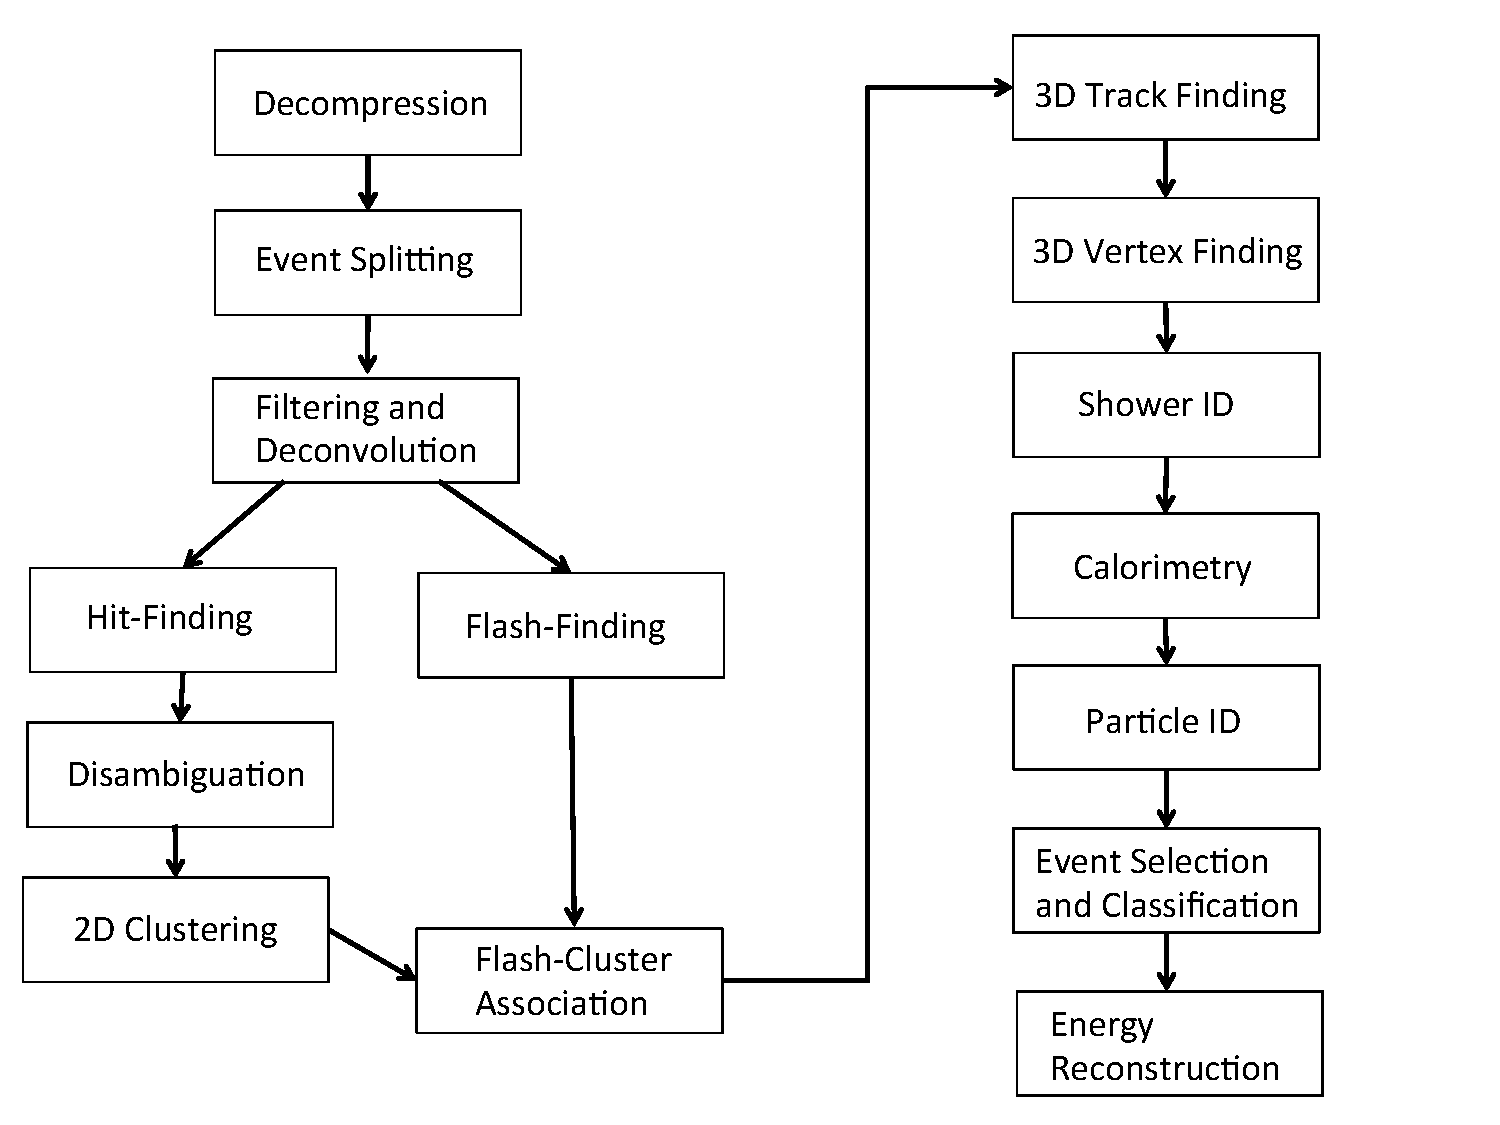
\includegraphics[width=0.7\textwidth]{fdrecoflowchart.pdf}
\end{cdrfigure}


\subsubsection{Signal Processing and Filtering}

A series of signal processing algorithms have been developed to
perform noise reduction and baseline subtraction on the digital
waveforms read out by Liquid Argon TPC detectors. 
These algorithms have been validated on data from 
\fixme{say where...}.

The TPC data are first uncompressed and put into local storage, one
channel at a time.  
%%%% MAYBE TOO MUCH DETAIL FOR CDR 
%In the case that the DAQ writes data records to persistent
%storage the correspond to inconveniently long time periods, the data may be split
%into smaller events at the readin stage.  At this stage, if an interaction is found
%to have taken place near the edge of the time corresponding to one record from the DAQ,
%the next one may be appended to make an offline event that corresponds more closely to
%what is required to analyze the interaction of interest.
\fixme{Single-phase paragraph follows:}
The detector response (bipolar vs. unipolar), and
electronics response functions are deconvoluted using a Fast Fourier
Transform (FFT) algorithm.  The FFT of the data are multiplied by the
inverse of the convolution kernel used in the simulation process,
multiplied by the frequency response of a noise filter, which
suppresses low-frequency and high-frequency noise.  It may be
necessary to filter unipolar signal components on the induction-plane
wires and handle these signals separately, in the case of partial
non-transparency of the induction planes, which might be unavoidable
near the wrapping boundaries.  The product of these is then
inverse-FFT'd back to the time domain to yield the deconvoluted
signals.  A computational speedup is achieved by packing data in
blocks that exceed thresholds plus nearby neighbors in time so that
the FFT only needs to see a fraction of the total ADC samples
collected in each event.

\fixme{Dual-phase paragraph follows - can it be merged with the single-phase material?}
Qscan also provides a set of methods for signal processing. 
The raw waveforms are first processed: this involves noise reduction as well as the subtraction of the baseline.
Hits, defined as signals that are discriminated from the noise, are identified and reconstructed.
In order to suppress noise without affecting the signal component too much, hence improving the signal to noise ratio, 
two different algorithms are used: the Fast Fourier Transform (FFT) filter, and the coherent noise subtraction algorithm.
A smooth cut-off, implemented with a Fermi potential, efficiently suppresses the noise without introducing artefact in the
time domain.
The coherent noise filter is implemented to remove identical noise patterns that are seen on larger sets of readout channels. 
Unlike in the case of the FFT filter, which directly suppresses the frequencies of single channels and thus reducing the signal bandwidth, the coherent noise filter ideally subtracts only the noise while keeping the signals unchanged.
After suppressing the noise, the (constant) pedestal of each waveform has to be computed and subtracted from each sample.


\subsubsection{TPC Hit Finding}

Once deconvoluted, raw ADC values trace out pulses, which are the best
estimates of when charge arrived on a particular electronics channel.
The widths of these pulses are determined by the detector resolution,
by diffusion, and by the intrinsic width of the charge formation
volume projected along the electric field dirction, which can be quite
long in the case of showers or tracks nearly aligned with the electric
field.  Multiple particles may contribute charge to the same pulse,
which is expected to be the case frequently in dense electromagnetic
showers, but can also occur from different particles leaving charge on
segments of the wire that are far apart, as the data from a wire do
not tell where along the wire the charge was deposited.  
Due to the wrapping of the induction-plane wires, pulses can contain charge
from opposite sides of the APA, but not for collection-plane signals.

\fixme{Single-phase paragraph follows:}
Hits are reconstructed pulses on each TPC DAQ channel.  Regions of
interest are identified in the stream of deconvoluted ADC samples, and
sums of Gaussian functions are fitted to the data using
MINUIT~\cite{minuit}.  The peak position, the width, the area, and the
sum of the deconvoluted ADC values corresponding to the fitted
Gaussian are recorded.  In the case that multiple overlapping Gaussian
fits are the best model of the data, the ADC sums are calculated for
the entire region of interest, and then divided among the contributing
hits proportional to their fit areas.  The efficiency of the hit
finder is shown in Figure~\ref{fig:hitfinderefficiency}.

\fixme{Dual-phase paragraph follows - can it be merged with the single-phase material?}
In Qscan, hits have to be extracted from the signal waveforms by means of a standard threshold discrimination. 
Due to changing noise conditions, the threshold is defined in relation to the measured RMS noise value, 
which is measured for each event and readout strip, using the pre-trigger samples.
In the general case there can be several close or overlapping tracks per event, producing a superposition of several signals/hits on a single readout strip. 
The shaping time constants of the preamplifiers are chosen such that double tracks being separated by a few $\mu s$ can be resolved.
The hit finding algorithms therefore extract multiple hit information by fitting the vaweform function of the signal.
The main parameters determined for the fitted hits are the hit time and the hit integral: 
together with the location of the corresponding readout channel, the hit time directly provides the information of the hit location in the considered view (projection), whereas the hit integral is related to the produced ionization charge and therefore provides the calorimetric information.


\subsubsection{Disambiguation}

A feature of liquid argon TPC geometries is that the location along a
wire at which charge is deposited is not measured, creating a
one-dimensional continuous ambiguity in the interpretation of the hits
on a wire.  As such, the planes of the TPC read out two-dimensional
``views'' of the three-dimensional events.  The wrapping of the
induction-plane wires in the DUNE APA design introduces another
discrete ambiguity -- the several wire segments that are connected
together to form a DAQ channel all contribute charge on that DAQ
channel, and it is not known from the wire's signal which of those
segments generated the charge.  This discrete ambiguity must be broken
before downstream reconstruction programs can do their work.

The detector geometry is chosen so that no induction-plane wire
crosses any collection-plane wire more than once, necessitating a
shallower induction-plane wire angle of 35.7$^\circ$.  The design from
the LBNE CDR~\cite{lbnecdr} proposed 44.3$^\circ$ and 45.7$^\circ$ as
the angles of the $U$ and $V$ wire planes, which necessitated
associating triplets of $U$, $V$, and $Z$ hits in order to break the
ambiguity.  Hit triplets consistent in drift time and with only one
possible combination of $U$, $V$, and $Z$ hits that intersect in one
position in space are determined to be ``trivially'' disambiguated.
More complicated cases where multiple possible hits in other planes
can be associated with a hit in a given plane, are disambiguated by
looking at nearby unambiguous hits and clustering them together.
Misassociation of hits in the three views, caused mainly by multiple
charge deposits arriving at the same time, can cause choosing the
incorrect wire segment.

The triplet-association algorithm is expected to work very well in the
35.7$^\circ$ geometry, by making few misassociations for the trivially
disambiguated sample.  Figure~\ref{fig:disambig} shows the
disambiguation performance for 6~GeV electrons and muons in the
35.7$^\circ$ far detector geometry.

\subsubsection{Optical Detector Signal Reconstruction}

The optical detector signals are reconstructed in two steps.  First, a
hit finder identifies signals on an individual channel, looking for
peaks while account for noise and pedestal.  Each hit is assigned a
total integrated charge and a time associated with the first peak,
since the SiPM signals are asymmetric and multiple individual photons
may get grouped together into a single hit if they are close in time.
Second, a flash finder groups together hits from across multiple
photon detectors which are coincident in time (a ``flash'' being a
source of light in the detector like the scintillation from the
passage of a charged particle).  Each flash has a total integrated
charge determined from its constituent hits as well as a
two-dimensional position determined by a charge-weighted average of
the positions of the photon detectors.  Since the photon detectors all
sit in a single plane, only two dimensional position reconstruction is
possible.  Once a flash is reconstructed, it becomes a candidate $t_0$
for objects reconstructed by the TPC.  If only a single track or
shower is present in the detector near the time of the flash, the
association is clear, but if there are multiple overlapping tracks a
likelihood-based method associates a TPC object with its best matching
flash.



\subsubsection{TPC Hit Clustering}

%After hit finding and disambiguation have completed, the hits in each plane are
%grouped togther in two-dimensional clusters, where the goal is to identify hits
%left by the interactions of individual particles with maximum efficiency and minimum overlap.
%``Fuzzy Cluster'' is a 2D clustering algorithm that proceeds in stages, making use of
%several algorithms developed outside of
%HEP.~\cite{flame}~\cite{ppht}~\cite{dbscan}. 

After the hit-finding and disambiguation stages have completed, a series of 
pattern recognition algorithms are applied to the 2D hits in order to identify 
the tracks and showers produced by individual final-state particles in an event.
In Liquid Argon TPC detectors, the pattern recognition stage must perform 
two functions in order to reconstruct 3D particles from 2D hits:
(a) identify the patterns of hits within each two-dimensional view
that correspond to individual particles; (b) match up hits and trajectories
between views in order to reconstruct particles as three-dimensional objects.
The development of automated pattern recognition algorithms for Liquid Argon 
TPC detectors is a relatively new field, but several 2D and 3D algorithms
have been implemented, using a range of different techniques.
For example, the ``Fuzzy Cluster'' package is a suite of algorithms that
performs two-dimensional clustering of hits using several techniques developed 
outside of HEP~\cite{flame}~\cite{ppht}~\cite{dbscan}.

A promising suite of pattern recognition algorithms, that provides fully 
automated reconstruction of 3D particle tracks and showers from 2D hits, 
is the PANDORA software development kit \fixme{INSERT PANDORA REFERENCE HERE}.
PANDORA implements a highly modular approach to pattern recognition,
in which the final-state particles within an event are reconstructed using 
a large chain of focused algorithms, each designed to identify and handle
a specific event topology. The reconstruction chain begins with a 
series of 2D pattern recognition algorithms that group together hits 
into clusters based on their topology and spatial proximity.
The next stage of the chain is 3D track reconstruction, 
which uses a rank-three tensor to match up all possible combinations 
of 2D clusters between the $U$, $V$, and $Z$views, and group together 
the best-matched triplets or doublets of clusters. If necessary, 
2D clusters are modified to improve the consistency of the 3D event. 
Once the 3D track trajectories have been identified, 
a series of vertex-finding algorithms are applied to the event,
which reconstruct the neutrino interaction vertex by analysing 
the 2D and 3D event topology. The remaining 2D clusters are then
used to reconstruct electromagnetic and hadronic showers,
first as extended 2D clusters, and then as 3D particles, 
using a similar procedure to 3D track reconstruction.
Finally, a neutrino event is formed by connecting together the 
reconstructed tracks and showers at the interaction vertex.

The PANDORA pattern recognition algorithms have been developed
using simulated neutrino interactions in the energy range 100\,MeV\,$-$\,25\,GeV.
Figure~\ref{fig:pandoraefficiency} shows the efficiency for reconstructing
the leading final-state lepton in 5\,GeV $\nu_{e}$ CC and $\nu_{\mu}$ CC interactions,
plotted as a function of momentum using the MicroBooNE detector geometry.
In both samples, the reconstruction efficiency increases rapidly with momentum,
rising above 90\% at 500\,MeV and reaching approxmately 100\% at 2\,GeV.
Figure~\ref{fig:pandoravertexresolution} shows the spatial resolution for
reconstructing the primary interaction vertex in 5\,GeV $\nu_{\mu}$ CC events,
projected onto the $x$, $y$ and $z$ axes. An estimate of the overall vertex 
resolution is obtained by taking the 68\% quantile of 3D vertex residuals, 
which yields 2.2\,cm (2.5\,cm) for $\nu_{\mu}$ CC ($\nu_{e}$ CC) events.


\fixme{CLUSTERING/PANADORA FOR LBNO (TWO VIEWS), taken from LGUNA-LBNO deliverables51 }

Algorithms specific for two views event reconstruction have been extensively developed as well. 
A preliminary 2D clustering is carried on similarly to what described above.
A first-pass hit clustering, using a nearest-neighbour algorithm and association algorithms is performed
on each projetion. Then primary vertex is found based on presumed beam direction and cluster positions/directions
(redundant information from all readout views is used to constrain the vertex location).
Primary final-state particles (seed-clusters) are finally identified, based on cluster length and proximity to vertex,
and each of the remanining non-seed cluster is associated with existing seed-clusters so that all energy deposits from a single final-state particle are grouped together.
At the end of this process, clusters not directly related to the vertex (either by pointing or position) 
will be associated with clusters coming from the vertex which are in close proximity, 
as long as there is not another vertex-related cluster nearby. 
Any remaining clusters far from the vertex will be removed, 
since it is assumed that these are actually related to an original final state particle, but we have been unable to make the association.

\fixme{Make the vertex resolution figure narrower!}

\begin{cdrfigure}[PANDORA reconstruction efficiency]{pandoraefficiency}
{Reconstruction efficiency of Pandora pattern recognition algorithms
 for the leading final-state lepton in 5\,GeV $\nu_{\mu}$ CC (left) and
 $\nu_{e}$ CC (right) neutrino interactions, plotted as a function of
 the lepton momentum. The reconstruction performance is evaluated
 using the MicroBooNE detector geometry. }
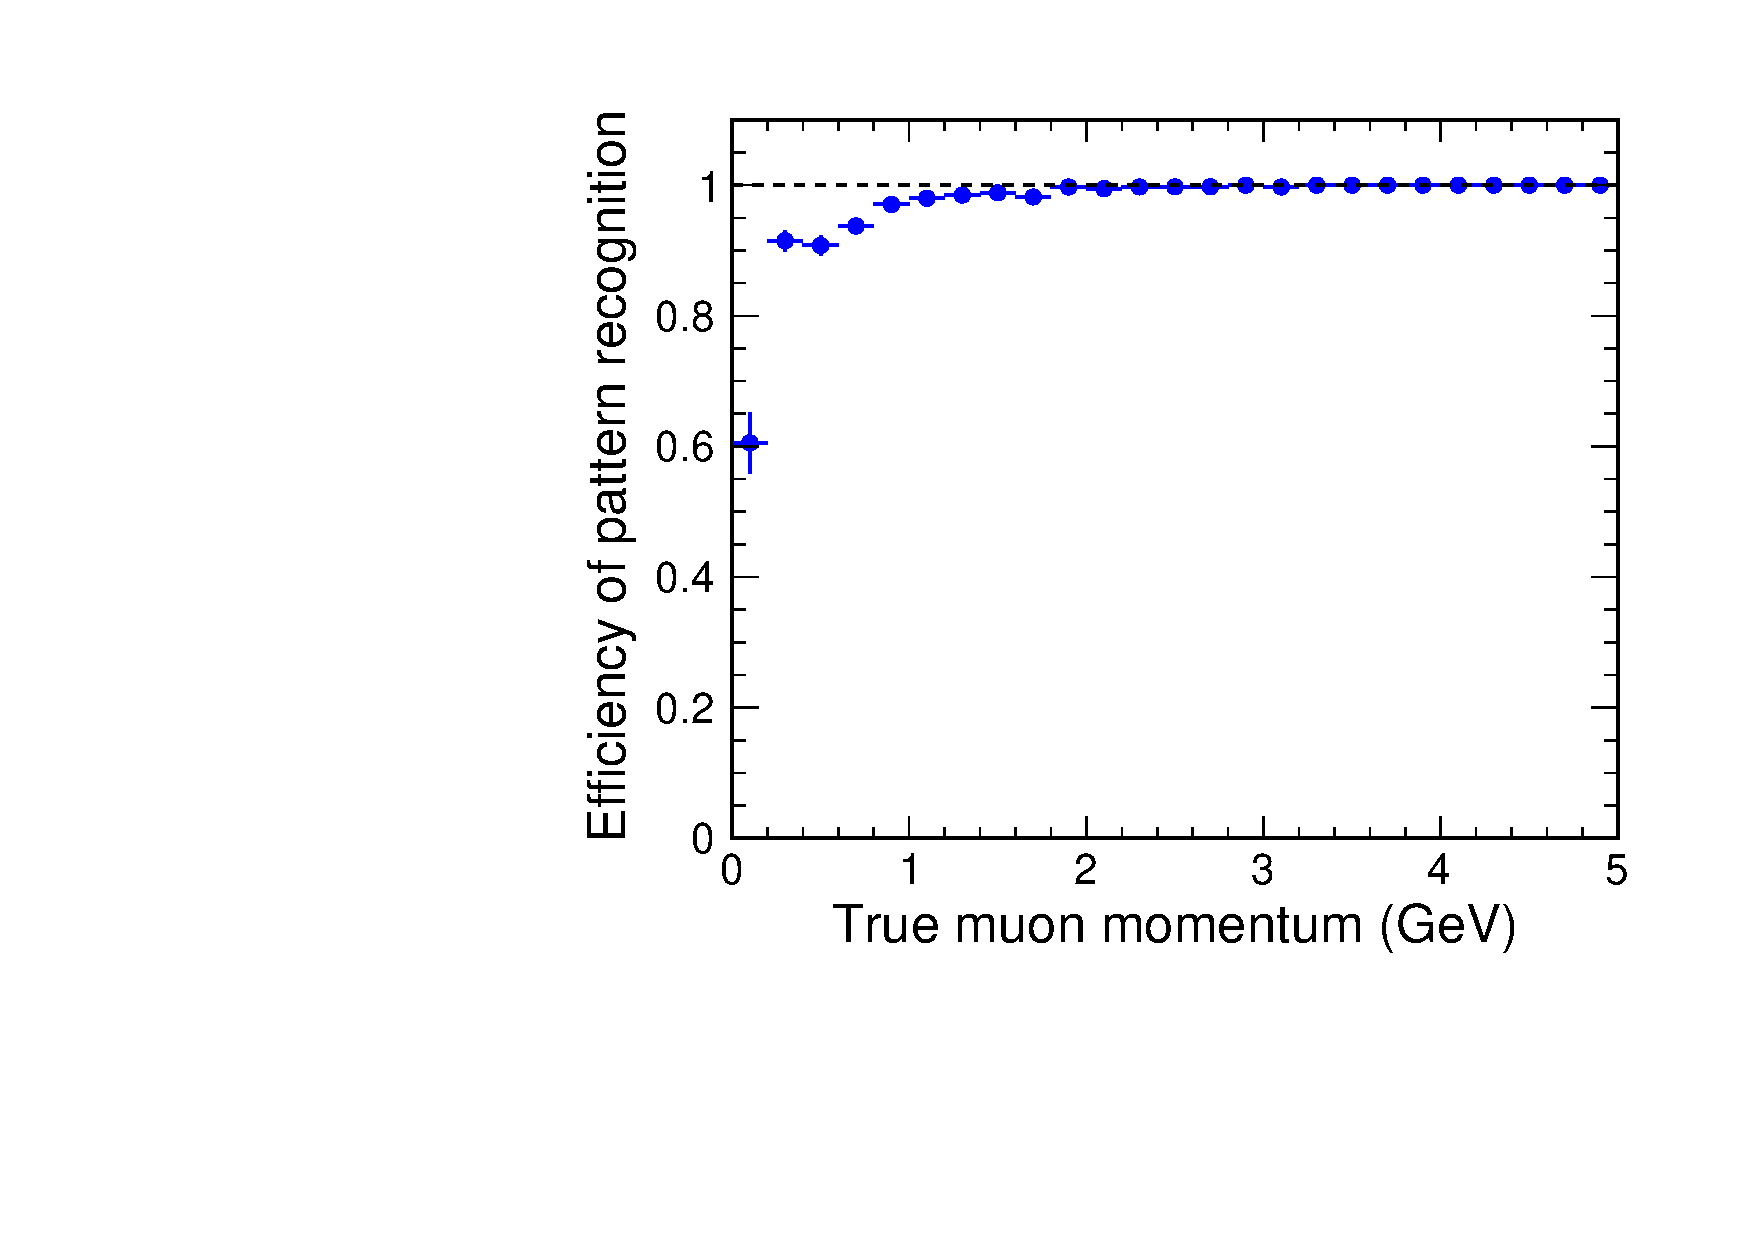
\includegraphics[width=0.49\textwidth]{pandora_uboone_efficiency_5GeV_numucc.pdf}
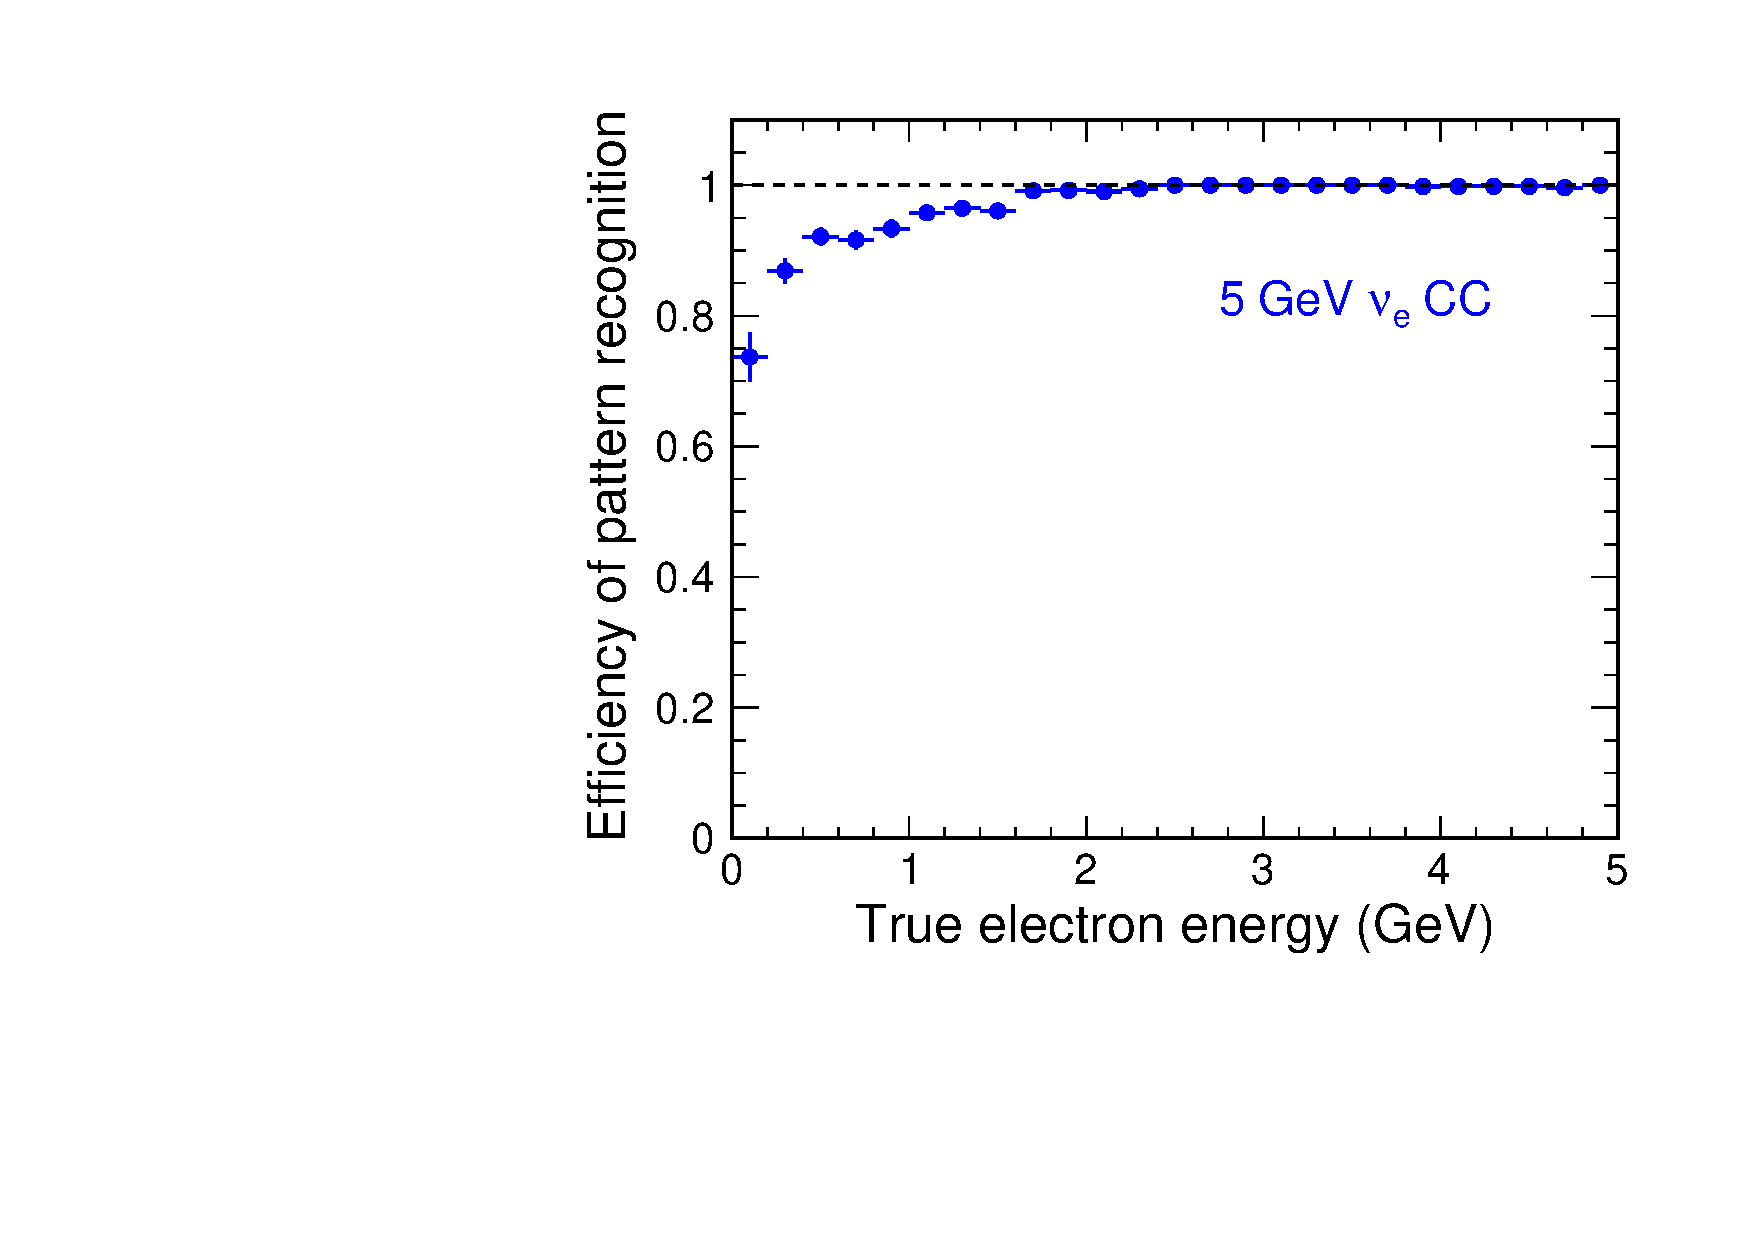
\includegraphics[width=0.49\textwidth]{pandora_uboone_efficiency_5GeV_nuecc.pdf}
\end{cdrfigure}

\begin{cdrfigure}[PANDORA vertex resolution]{pandoravertexresolution}
{Distribution of 2D residuals between reconstructed and simulated interaction
 vertex for 5\,GeV $\nu_{\mu}$ CC interactions in the MicroBooNE detector.
 The $x$ axis is oriented along the drift field, the $y$ axis runs parallel 
 to the collection plane wires, and the $z$ axis points along the beam direction.}
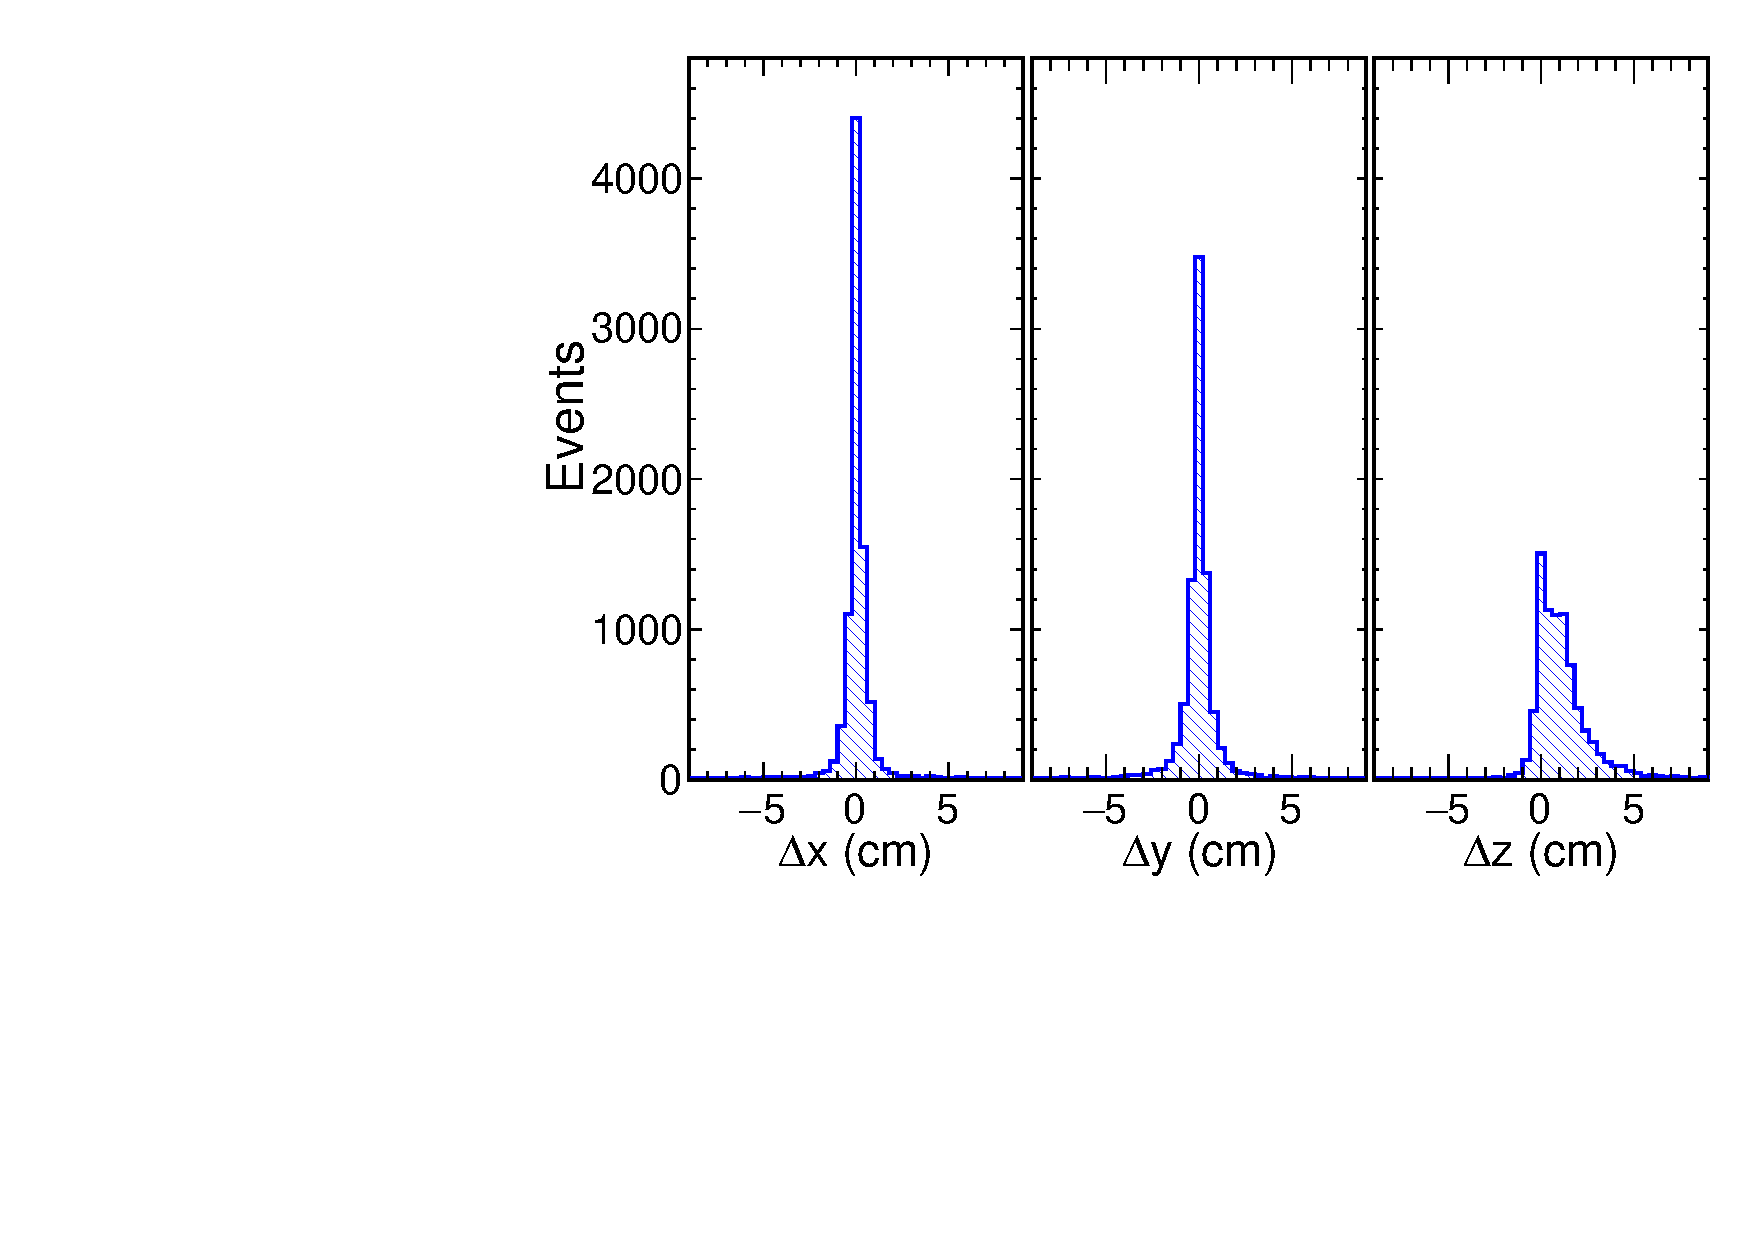
\includegraphics[width=\textwidth]{pandora_uboone_vertex_resolution.pdf}
\end{cdrfigure}


\subsubsection{Track Fitting}

%%%%% Section taken from the LArSoft NIM article -- to rephrase

The track reconstruction problem in a liquid argon TPC is divided
into: trajectory reconstruction, and track parameter estimation.
Hits are the input data for track reconstruction. Hits represent a
one-dimensional measurement of a track (the drift time) on a
measurement surface defined by the charge drift direction and the
readout wire. Hits from multiple views may be combined into
three-dimensional space points. Three dimensional track reconstruction
can proceed from space points or directly from hits.

The Kalman filter algorithm~\cite{kalman} has been widely used in high
energy physics for track reconstruction. The Kalman filter provides an
elegant mathematical solution to the problem of finding an optimal
track description from a collection of candidate measurements that are
hits or space points, especially in cases where the number of
measurements is much larger than the five parameters needed to specify
a track on a surface.  The Kalman filter can be used for both pattern
recognition and parameter estimation.

\fixme{Can we say something about current status or performance?}

%%%% MAYBE TOO MUCH DETAIL FOR CDR 

%The measurement surfaces in liquid argon TPCs intersect, which
%means there is no predetermined order in which the measurement
%surfaces should be visited.  To prevent back-and-forth tracking, which
%would overestimate propagation noise, such as multiple Coulomb
%scattering, the LArSoft Kalman filter chooses the measurement
%surfaces associated with one view as primary, and visits these
%surfaces in their natural predetermined order.  Hits from views other
%than the primary view are added to the track by treating the
%propagation from the track surface to the non-parallel hit measurement
%surface as part of the measurement function.  This measurement
%propagation is always done using a linear approximation as is the
%measurement function, and is done without propagation noise.

%The LArSoft Kalman filter does not use a branching track model. Hit
%selection for the LArSoft Kalman filter is implemented such that at
%each measurement surface, the filter accepts either zero or one
%hit. 

%If the Kalman filter assigns the wrong hit to a track, the track may follow
%the wrong road (e.g. a delta ray), or the track may otherwise end
%prematurely.  Fixing broken tracks relies on a track-stitching
%algorithm that runs after the initial Kalman filter reconstruction.

\subsubsection{Shower Measurement}

%%%%% Section taken from the LArSoft NIM article -- to rephrase

The electromagnetic shower algorithms have two
steps. The first is a post-clustering stage which examines the
existing clusters in terms of their 2D parameters to determine whether
the clusters are shower-like or track-like. 
The selected shower-like clusters are examined to assign starting points,
directions and angles in the wire-time plane. The second step is 
3D shower reconstruction, which
matches the 2D clusters between views in order to obtain 3D shower axes and start points.
These 3D parameters allow the calculation of the shower energies and charge
depositions at the starts of the showers, which are used in particle
identification. 

\fixme{Can we say something about current status or performance?}

\subsubsection{Calorimetry}

%%%%% Section taken from the LArSoft NIM article -- to rephrase

As charged particles traverse a volume liquid argon, they deposit
energy through ionization and scintillation. It is important to
measure the energy depotion as it provides information on particle
energy and species. The algorithm for reconstructing the ionization
energy in LArSoft is optimized for line-like tracks and is being
extended to showers. 
For each hit on a reconstructed track, the hit area or amplitude, in ADC counts, is
converted to the charge $Q_{det}$, in fC units, on the wire using an
ADC to fC conversion factor that is determined by muons or test-stand
measurements. To account for the charge loss along the drift due to
impurities, a first correction is applied to $Q_{det}$ to get the free
charge after recombination $Q_{free} = Q_{det}/e^{-t/\tau_{e}}$, where
$t$ is the electron drift time for the hit and $\tau_{e}$ is the
electron lifetime measured by the muons or purity monitors. The charge
$Q_{\rm{free}}$ is divided by the track pitch $dx$, which is defined as the
dot production of track direction and the direction normal to the wire
direction in the wire plane, to get the $dQ_{\rm{free}}/dx$ for the
hit. Finally, to account for charge loss due to recombination, also
known as ``charge quenching'', a second correction is applied to
convert $dQ_{\rm{free}}/dx$ to $dE/dx$ based on the modified Box's model
\cite{box} or Birks's model\cite{birks}. The total energy
deposition from the track is obtained by summing the $dE/dx$ from each
hit: $\sum\limits_{i}^{\rm{all\ hits}}(dE/dx)_{i}\cdot dx_{i}$.

\fixme{Borrow performance plot from LBNE Science Opportunities document?}

\subsubsection{Particle ID}

%%%%% Section taken from the LArSoft NIM article -- to rephrase

If the incident particle stops in the LArTPC active volume, the energy
loss, $dE/dx$, as a function of the residual range ($R$), the path
length to the end point of the track, is used as a powerful method for
particle identification. There are two methods in LArSoft to determine
particle species using calorimetric information. The first method
calculates four $\chi^{2}$ values for each track by comparing measured
$dE/dx$ versus $R$ points to the proton, charged kaon, charged pion
and muon hypotheses and identifies the track as the particle that
gives the smallest $\chi^{2}$ value. The second method calculates the
quantity ${\rm{PIDA}} = <A_{i}> = <(dE/dx)_{i}R_{i}^{0.42}>$ \cite{box},
which is defined to be the average of $A_{i} =
(dE/dx)_{i}R_{i}^{0.42}$ over all track points where the residual
range $R_{i}$ is less than 30 cm. The particle species can be
determined by making a selection on the PIDA value.

\fixme{Current results?}

\subsubsection{Calibration}

In order to meet the requirements of high detection efficiency, efficient and
pure particle identification, excellent energy resolution, and small systematic
uncertainties on these performance parameters, calibrations of the detector
will be needed.  {\it In situ} calibration techniques using data collected by the FD
under identical conditions as used for physics analyses are the most desirable.
These include studying cosmic-ray events and non-fiducial interactions.  But not
all performance measures can be calibrated in this way.  A laser calibration system
will constrain the detector alignment as well as measure any residual space-charge effects
(which are expected to be very small underground), as well as provide timing calibraiton
and crosscheck the response to drifting charge.  The electronics will be outfitted with
charge-injection calibration systems so that non-uniformities in the electronics response
can be corrected in a time-dependent fashion.  The response to charged particles of known
energy and particle type will rely on test-beam data from LArIAT and the CERN test
experiments WA104 and WA105.


